\chapter{TikZ 基础}

参考 Introduction to TikZ\footnote{\url{https://www.math.univ-angers.fr/~naie/varia/tutorial_7.pdf}}.

\section{简介: 绘图与画布}

TikZ 是 {\LaTeX} 绘图工具 PGF 的前端层\footnote{PGF ("portable graphics format") is the basic layer, providing a set of basic commands for producing graphics, and TikZ ("TikZ ist kein Zeichenprogramm" or "TikZ is not a Drawing program") is the frontend layer with a special syntax, making the use of PGF easier.}. 
TikZ 绘图命令需要在 \textcolor{magenta}{\itshape tikzpicture} 环境中, 并且绘图命令要用分号结束. 

\begin{minted}{latex}
\begin{tikzpicture}[<options>]
  <tikz commands>
\end{tikzpicture}
\end{minted}

如\footnote{为了方便起见, 这里显示代码, 并渲染之.}:
\begin{latexcode}{nobox}
\begin{tikzpicture} 
  \draw (0,0) rectangle (1em,1em); 
\end{tikzpicture}
\end{latexcode}
或者简单写成:
\tikz \draw (0,0) rectangle (1em,1em);,或:
\tikz[baseline=1ex] \draw (0,0) rectangle (1em,1em);, 注意后者设置了 {\ttfamily baseline}.

\subsection{坐标与点}

下面的例子中, 使用 {coordinate}
\footnote{{coordinate} 是 {path coordinate} 的缩写} 定义点并以该点为圆心画圆:
\begin{latexcode}{nobox}
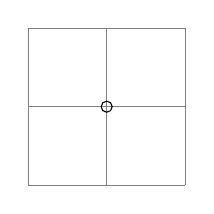
\begin{tikzpicture}
  \draw [help lines] (-1,-1) grid (1,1);
  \coordinate (A) at (0,0);
  \draw (A) circle (2pt);
\end{tikzpicture}
\end{latexcode}

\subsection{坐标系}

有两种坐标系的定义方式:

显式 explicitly: 如 {\ttfamily (canvas cs:x=2, y=0)}

隐式 implicitly: 如笛卡尔坐标 {\ttfamily (2,0)} 或极坐标 {\ttfamily (45:1.5)}

\subsection{循环}

\mint{latex}|\foreach \i [options] in {<list>}{<commands>};|

\begin{latexcode}{nobox}
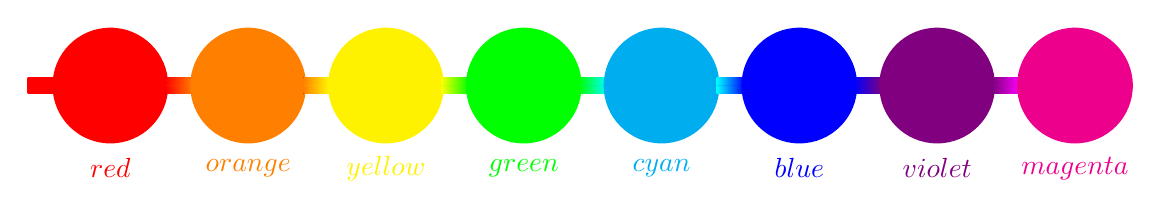
\begin{tikzpicture}[scale=0.35]
  \foreach \rC [count=\j from 0, remember=\rC as \lC (initially red)] in 
  {red, orange, yellow, green, cyan, blue, violet, magenta}{
    \fill[left color=\lC, right color=\rC] (5*\j, -.3) rectangle +(1, .6);
    \fill[\rC] (5*\j, 0) -- ++(3, 0) circle (2.1) node at ++(0, -3) {$\rC$}; 
  }
\end{tikzpicture}
\end{latexcode}

\section{点与曲线}

\subsection{路径 Path 及其属性}

路径 Path 是一些列直线或曲线的点. 创建路径的命令是 {path <specifications>}, 为了使路径可见, 我们需要增加
动作 {\ttfamily draw}\footnote{{draw} 是 {path[draw] 的缩写.}}, 如: 

\begin{latexcode}{nobox}
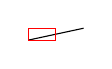
\begin{tikzpicture}
  \path[draw] (0,0) -- (2em,1ex) coordinate (A);
  \path[draw,red] (0,0) rectangle (1em,1ex);
\end{tikzpicture}
\end{latexcode}

{\ttfamily <specifications>} 是一组路径操作或属性, 如:

\begin{tabular}{cc}
\toprule
operations/attributes & descriptions \\
\midrule
{\ttfamily -- (0,0)} & line to \\
{\ttfamily to (0,0)} & line to \\
{\ttfamily let ... in} & 求值运算, 结果存入 {x.}, {y.}, {p.} \\
{\ttfamily [draw]} & 绘图 \\
{\ttfamily color=blue} & 设置颜色 \\
{\ttfamily line width=2pt} & 设置线宽 \\
{\ttfamily coordinate} & 定义点坐标 \\
{\ttfamily node} & 添加文本 (注意不是路径的一部分) \\
{\ttfamily pic} & 引入小的图片和替代 node \\
\bottomrule
\end{tabular}

\begin{latexcode}{nobox}
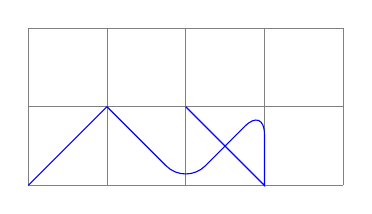
\begin{tikzpicture}
  \draw [help lines] (0,0) grid (4,2);
  \draw[blue] (0,0) -- (1,1) {[rounded corners=10pt] -- (2,0) -- (3,1)}
  -- (3,0) -- (2,1);
\end{tikzpicture}
\end{latexcode}

% \subsection{相对坐标}

% \begin{tabular}{cc}
% \toprule
% form & descriptions \\
% \midrule
% {\ttfamily {-}{-} (x,y)} & 绝对坐标 \\  % {-}{-} 防止变成一个 - 号
% {\ttfamily {-}{-} +(x,y)} & 相对第 1 个绝对坐标 \\
% {\ttfamily {-}{-} ++(x,y)} & 相对前一个坐标 \\
% \bottomrule
% \end{tabular}

% \begin{latexcode}{nobox}
% \begin{tikzpicture}
%   \draw [help lines] (-4,-4) grid (4,4);
%   \draw [-latex] (-4.5,0) -- (4.5,0) node[below] {$x$};
%   \draw [-latex] (0,-4.5) -- (0,4.5) node[left] {$y$};
%   \draw (0,0) node [below left] {$O$};
%   \draw [thick,blue] (0,1) -- (2,1) -- (-2,1.5) -- (-1,-1) -- cycle;
%   \draw [thick,red] (0,1) -- +(2,1) -- +(-2,1.5) -- +(-1,-1) -- cycle; 
%   \draw [thick,green] (0,1) -- ++(2,1) -- ++(-2,1.5) -- ++(-1,-1) -- cycle;
%   \draw [thick,magenta] (0,0) -- ++(-45:1) -- ++(60:2) -- cycle;
% \end{tikzpicture}
% \end{latexcode}

% \subsection{贝塞尔曲线 Bézier}

% \begin{latexcode}{nobox}
% \begin{tikzpicture}
%   \draw [help lines] (0,0) grid (3,3);
%   \draw [thick,blue] (0,0) -- (1,2) .. controls (1.5,3) .. (3,0);
% \end{tikzpicture}
% \end{latexcode}

% \subsection{操作路径 Path}

% {\ttfamily draw, fill, shade, clip} 等

% \section{坐标计算}

% {\ttfamily ($(p1)!c!(p2)$)}

% {\ttfamily ($(p1)!c!angle:(p2)$)}

% 垂直平分线:
% \begin{latexcode}{nobox}
% % \usetikzlibrary{calc}
% \begin{tikzpicture}
%   \coordinate (A) at (0,0);
%   \coordinate (B) at (4,1);
%   \coordinate (M) at ($(A)!0.5!(B)$);
%   \draw (A) -- (B);
%   \draw [blue] ($(M)!2!90:(B)$) -- ($(M)!2!-90:(B)$);
%   \foreach \p in {A,B,M}
%     \draw (\p) circle (2pt);
%   \draw (A) node [below left] {$A$};
%   \draw (B) node [below right] {$B$};
%   \draw (M) node [below right] {$M$};
% \end{tikzpicture}
% \end{latexcode}

% \begin{latexcode}{nobox}
% % \usetikzlibrary{math}
% \begin{tikzpicture}[evaluate={%
%     int \i;
%     for \i in {0, ..., 10}{\r{\i} = .1*(\i+1);}; 
%   }]
%   \foreach \i [evaluate=\i as \tmp using \i*10] in {0,...,10}{% 
%     \filldraw[white, fill=magenta!\tmp!cyan]
%     ($(0, 0)!\i/12!\i*18:(5, -1)$) circle (\r{\i});
%   }
% \end{tikzpicture}
% \end{latexcode}

% \subsection{投影}

% {\ttfamily ($(p1)!p!(p2)$)}

% 三角形的高线:
% \begin{latexcode}{nobox}
% % \usetikzlibrary{calc}
% \begin{tikzpicture}
%   \coordinate (A) at (0,0);
%   \coordinate (B) at (5,-1);
%   \coordinate (C) at (2,3);
%   \draw[thick] (A) -- (B) -- (C) -- cycle;
%   \draw[blue,thin] 
%     (A) -- ($(B)!(A)!(C)$) coordinate (A')
%     (B) -- ($(A)!(B)!(C)$) coordinate (B')
%     (C) -- ($(A)!(C)!(B)$) coordinate (C');
%   \foreach \p in {A,B,C,A',B',C'}
%     \draw (\p) circle (2pt);
%   \draw (A) node [below left] {$A$};
%   \draw (B) node [below right] {$B$};
%   \draw (C) node [above] {$C$};
%   \draw (A') node [above right] {$A'$};
%   \draw (B') node [above left] {$B'$};
%   \draw (C') node [below] {$C'$};
% \end{tikzpicture}
% \end{latexcode}

% Simson 线:
% \begin{latexcode}{nobox}
% % \usetikzlibrary{calc}
% \begin{tikzpicture}
%   \coordinate (A) at (-10:2);
%   \coordinate (B) at (55:2);
%   \coordinate (C) at (170:2);
%   \coordinate (P) at (-80:2);
%   \draw [magenta] (0,0) circle (2);
%   \draw[thick] (A) -- (B) -- (C) -- cycle;
%   \draw[blue,thin] 
%     (P) -- ($(B)!(P)!(C)$) coordinate (A')
%     (P) -- ($(A)!(P)!(C)$) coordinate (B')
%     (P) -- ($(A)!(P)!(B)$) coordinate (C');
%   \draw[red,thick] (A') -- (C');
%   \foreach \p in {A,B,C,A',B',C',P}
%     \draw (\p) circle (2pt);
%   \draw (A) node [right] {$A$};
%   \draw (B) node [above right] {$B$};
%   \draw (C) node [left] {$C$};
%   \draw (A') node [above] {$A'$};
%   \draw (B') node [above right] {$B'$};
%   \draw (C') node [above right] {$C'$};
%   \draw (P) node [below right] {$P$};
% \end{tikzpicture}
% \end{latexcode}

% \subsection{交点}

% \subsubsection*{第 1 形式}

% \mint{latex}|name intersections={of=<curve1> and <curve2>, name=<prefix>}|

% 如果有非封闭图形, 可以作为排序的图形 {\ttfamily sort by=curve name}:

% \begin{latexcode}{nobox}
% \begin{tikzpicture}
%   \draw [help lines] (-2,-2) grid (2,2);
%   \draw [name path=circle] (0,0) circle (2);
%   \draw [name path=line] (-2,-2) -- (3,0);
%   \path [name intersections={of=circle and line, name=iP, sort by=line}];
%     \foreach \j/\pos in {1/below, 2/below right}{%
%   \filldraw[red] (iP-\j) circle (2pt) node[\pos, black] {$I_{\j}$}; }
% \end{tikzpicture}
% \end{latexcode}

% \subsubsection*{第 2 形式}\mint{latex}|name intersections={of=<curve1> and <curve2>, by=<points>}|

% \begin{latexcode}{nobox}
% \begin{tikzpicture}
%   \draw [help lines] (-2,-2) grid (2,2);
%   \draw [name path=circle] (0,0) circle (2);
%   \draw [name path=curve] (-2,-2) .. controls (-0.5,-1) .. (0,0)
%     .. controls (0.5,1) .. (2,2);
%   \path[name intersections={of=circle and curve, by={A, B}, sort by=curve}];
%   \foreach \P/\pos in {A/below, B/above}{%
%     \filldraw[blue] (\P) circle (2pt) node[\pos] {$\P$};
%   }
% \end{tikzpicture}
% \end{latexcode}

% \subsubsection*{第 3 形式}\mint{latex}|name intersections={of=<curve1> and <curve2>, name=<prefix>, total=\t}|

% \begin{tikzpicture}
%   \draw[help lines] (-2,-2) grid (2,2);
%   \draw[name path=circle] (0,0) circle (2);
%   \draw[rotate=-45,name path=ellipse] (-1,-1) ellipse (3 and 1);
%   \fill[name intersections={of=circle and ellipse, name=I, total=\t}] 
%     [blue] \foreach \j in {1, ..., \t}{%
%       (I-\j) circle (2pt) node[above right] {$I_\j$} 
%     };
% \end{tikzpicture}

% \section{几何变换}

% 几何变换有:

% \begin{itemize}
%   \item {\ttfamily rotate=<angle in degree>}
%   \item {\ttfamily xshift=<length, yshift=<length>}
%   \item {\ttfamily shift=<\{vector\}>} 注意花括号
%   \item {\ttfamily xscale=<factor>, yscale=<factor>}
%   \item {\ttfamily scale=<factor>}
% \end{itemize}

% \begin{latexcode}{nobox}
% \begin{tikzpicture}
%   \draw[help lines] (-2,-2) grid (4,4);
%   \draw[thick,blue] 
%     (-1,0) -- (0,0) -- (60:1) .. controls (1,0) .. (2,0);
%   \draw[thick,red,rotate=45] 
%     (-1,0) -- (0,0) -- (60:1) .. controls (1,0) .. (2,0);
%   \draw[thick,orange,shift={(2,.5)}] 
%     (-1,0) -- (0,0) -- (60:1) .. controls (1,0) .. (2,0);
%   \draw[thick,cyan,rotate=45,shift={(2,.5)}] 
%     (-1,0) -- (0,0) -- (60:1) .. controls (1,0) .. (2,0);
%   \draw[thick,magenta,shift={(2,.5)},rotate=45] 
%     (-1,0) -- (0,0) -- (60:1) .. controls (1,0) .. (2,0);
% \end{tikzpicture}
% \end{latexcode}

% \section{箭头}

% \tikz \draw[->] (0,0) -- (1,0);

% \tikz \draw[-latex] (0,0) -- (1,0);

% \section{Node}

% A node is typically a rectangle or circle or another simple shape with some text on it. Nodes are added to paths using the special path operation {\ttfamily node}. {\itshape Nodes are not part of the path itself}. Rather, they are added to the picture just before (with the attribute {\ttfamily behind path}) or after the path has been drawn.

% Coordinate transformations do not apply to a node. Its anchor remains the same. To achieve a translation for example, the shift command must be placed inside the node’s name parentheses.

% \subsection{定义 Node}

% Thepathoperation...node[<options>] (nName) at (a,b) {content}...;createsanode for the current path, i.e. writes down the content at the point (a,b) with some node options and name nName. The node options or attributes have no effect outside the node; they control its

% \begin{itemize}
%   \item position with respect to the elements of the path – anchor
%   \item appearance
%   \item label.
% \end{itemize}

% \begin{latexcode}{nobox}
% \begin{tikzpicture}
%   \path (0, 0) coordinate (A) node[below left] {$A$}; 
%   \path (3, 2) coordinate (B) node[below right] {$B$}; 
%   \draw (A) to[out=-30, in=180] 
%     node[draw, red, pos=.5, above left] {content}
%     node[draw, blue, pos=.5] {content} (B); 
%   \draw[fill=white] (A) circle (2pt) (B) circle (2pt);
% \end{tikzpicture}
% \end{latexcode}

% \section{plot}

% {\ttfamily addplot, addplot3} 需要 pgfplots 宏.

% \subsection{从文件中读取数据}

% \begin{latexcode}{nobox}
% \begin{tikzpicture}
%   \begin{axis}
%   \addplot table [x=column 1, y=column 2, col sep=comma] {table.csv};
%   \end{axis}
% \end{tikzpicture}
% \end{latexcode}

% \subsection{绘制函数图像}

% 可以使用 {\ttfamily plot} , 可以使用 {\ttfamily addplot} \footnote{\url{https://pressbooks.bccampus.ca/introtolatex/chapter/packages/}}:

% \begin{latexcode}{nobox}
% \begin{tikzpicture}
%   \draw[help lines] (-4,-4) grid (4,4);
%   \draw[-latex] (-4.5,0) -- (4.5,0) node [below] {$x$};
%   \draw[-latex] (0,-4.5) -- (0,4.5) node [left] {$y$};
%   \draw (0,0) node [below left] {$O$};
%   \draw[domain=-3:3, smooth, variable=\x, red] 
%     plot ({\x}, {\x*\x/5}) node[above] {$y=\cfrac{x^2}{5}$};
%   \draw[domain=-3:3, samples=20, variable=\x, blue] 
%     plot ({\x}, {-cos(2*deg(\x))-1}) node[above] {$y=-\cos{2x}-1$};
%   \draw[variable=\t, domain=-1.6:1.6, samples=50]
%     plot (\t*\t-1, {\t*(\t*\t-1)}) node[above] {$y^2=x^3+x^2$};
% \end{tikzpicture}
% \end{latexcode}

% \begin{latexcode}{nobox}
% \begin{tikzpicture}
%   \begin{axis}[
%     axis lines = left,
%     xlabel = $x$,
%     ylabel = {$f(x)$}
%   ]
%   \addplot [ 
%     domain=-10:10,
%     samples=30,
%     color=blue
%   ]{x^2 + 2*x + 1};
%   \addplot [ 
%     domain=-10:10,
%     samples=40,
%     color=red
%   ]{20*sin(pi*x^2)};
%   \end{axis}
% \end{tikzpicture}
% \end{latexcode}

% \subsection{三维图}

% \begin{latexcode}{nobox}
% \begin{tikzpicture}[scale=2]
%   \begin{axis}[
%     %title={$f(x,y)=y\exp(-x^2-\|y\|)$},
%     hide axis,
%     colormap/cool,  
%   ]
%   \addplot3[
%     surf, 
%     domain=-3:3, 
%     domain y=-3:3, 
%     samples=40
%   ]{y*exp(-x*x-abs(y))};
%   \end{axis}
% \end{tikzpicture}
% \end{latexcode}

% \begin{latexcode}{nobox}
% \begin{tikzpicture}[scale=2]
%   \begin{axis}[
%     %title={$f(x,y)=\cfrac{\sin{\sqrt{x^2+y^2}}}{\sqrt{x^2+y^2}}$},
%     hide axis,
%     colormap/cool,
%   ]
%   \addplot3[
%     mesh,
%     samples=50,
%     domain=-8:8,
%   ]{sin(deg(sqrt(x^2+y^2)))/sqrt(x^2+y^2)};
%   \end{axis}
% \end{tikzpicture}
% \end{latexcode}

% \section{pic}

% \subsection{标记角}

% \begin{latexcode}{nobox}
% \begin{tikzpicture}
%   \draw
%     (3,-1) coordinate (a) node[right] {$A$}
%     -- (0,0) coordinate (b) node[left] {$B$}
%     -- (2,2) coordinate (c) node[above right] {$C$}
%     pic["$\alpha$", draw=orange, <->, angle eccentricity=1.2, angle radius=1cm]
%     {angle=a--b--c};
% \end{tikzpicture}
% \end{latexcode}


